%
% singularities.tex -- -- XXX
%
% (c) 2008 Prof Dr Andreas Mueller
%
\section{Entstehung von Singularitäten}
Die Lösung einer partiellen Differentialgleichung hängt entscheidend
vom Verlauf der Charakteristiken ab. Treffen sich zwei Charakteristiken
in einem Punkt, ist die Lösung nicht eindeutig bestimmt. Die Lösung
ist also nur solange bestimmt, als sich die Charakteristiken nicht überschneiden.
Andernfalls treten Singularitäten in der Lösung auf.

Als Beispiel betrachten wir die nichtlineare Gleichung 
\begin{equation}
\frac{\partial u}{\partial t}+u\frac{\partial u}{\partial x}=0.
\label{wellenichtlinear}
\end{equation}
mit der Anfangsbedingung 
\[
u(0,x_0)=g(x_0)=e^{-4(x_0-\frac12)^2}.
\]
Nach der Methode der Charakterisitiken brauchen wir eine Lösungskurve
des Vektorfeldes
\[
\begin{pmatrix}
1\\
u\\
0
\end{pmatrix}
\]
durch den Punkt $(0,x_0, z_0)$, also eine Lösung des Differentialgleichungssystems
\[
\left.
\begin{aligned}
\frac{d}{d\tau} t(\tau)&=1\\
\frac{d}{d\tau} x(\tau)&=z(\tau)\\
\frac{d}{d\tau} z(\tau)&=0
\end{aligned}
\quad
\right\}
\qquad
\Rightarrow
\qquad
\left\{
\quad
\begin{aligned}
t(\tau)&=\tau\\
z(\tau)&=z(0)\\
x(\tau)&=z(0)\tau +x(0)
\end{aligned}
\right.
\]
Der Parameter $\tau$ hat also die Bedeutung von $t$.
Die Lösungsfläche ist somit
\[
(t,x_0)\mapsto
\begin{pmatrix}
t\\
g(x_0)t+x_0\\
g(x_0)
\end{pmatrix}.
\]
Die Charakteristiken in der $x$-$y$-Ebene sind Geraden mit einer
Steigung, die von $g(x_0)$ abhängt. Je grösser $g(x_0)$ ist, desto
``schneller'' bewegt sich die Integralkurve nach ``rechts''. Grosse
Werte der Anfangsbedingung können also die kleinen Wert überholen,
dabei entsteht eine Singularität.

Zur Zeit $t$ hat die Lösungsfunktion die Parameterdarstellung
\[
x_0\mapsto (g(x_0)t+x_0,g(x_0))
\]
die Graphen in Abbildung~\ref{g} zeigen, wie sich die Lösungskurve
mit zunehmender Zeit entwickelt.
Es ist offensichtlich, dass für genügend grosse Zeit $t$ die
Lösungsfläche nicht mehr als Graph einer Funktion $u(t,x)$ derstellbar ist.
\begin{figure}
\begin{center}
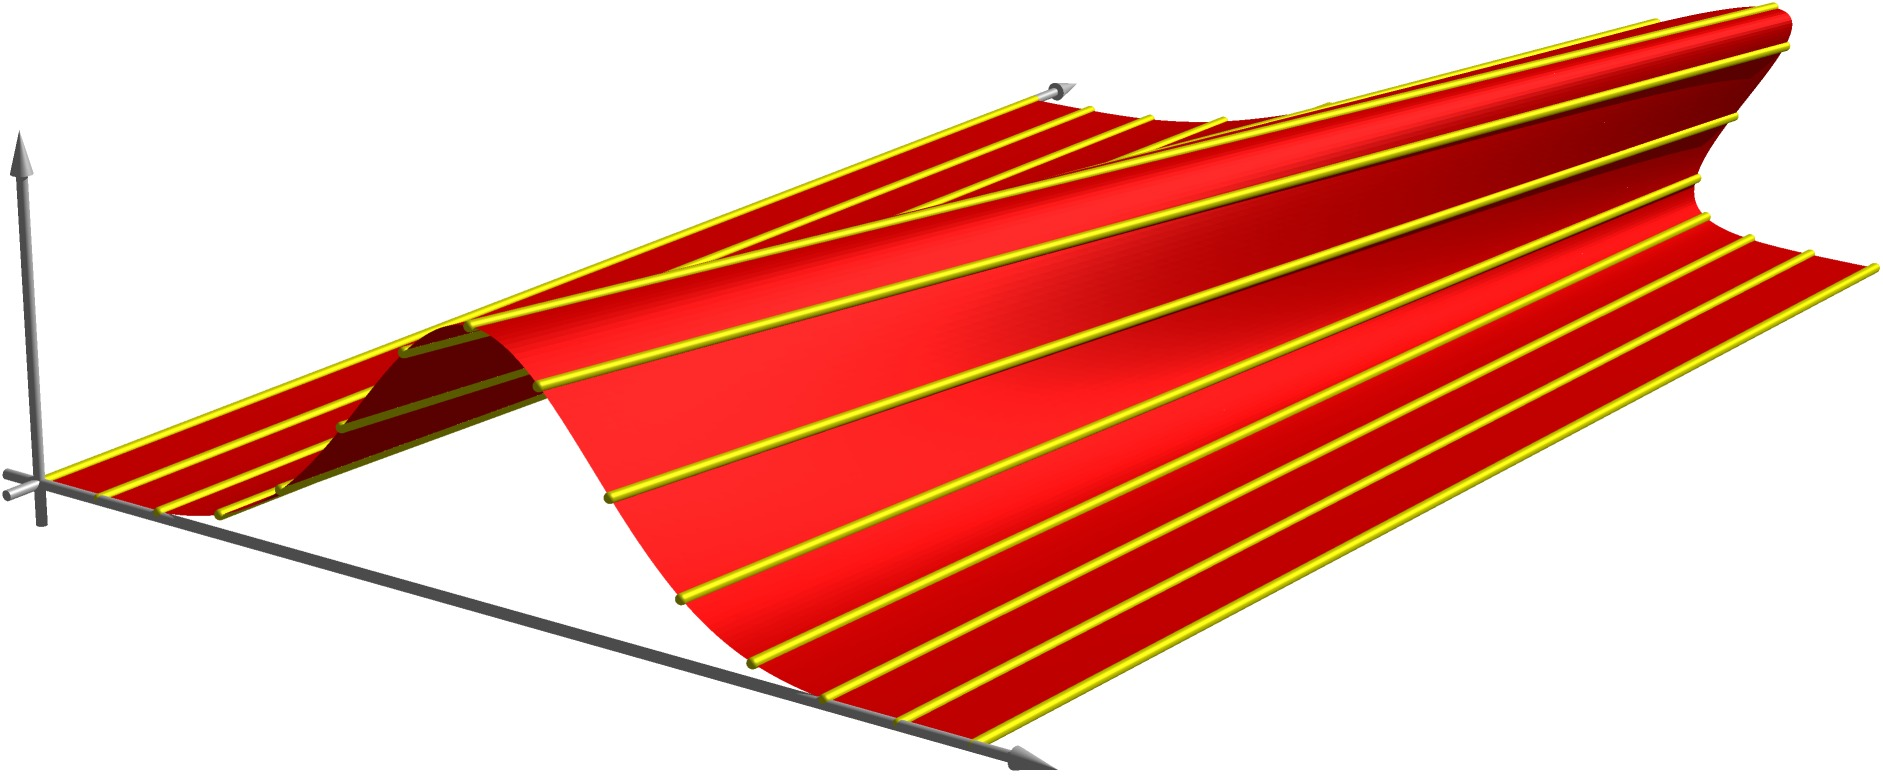
\includegraphics[width=\hsize]{../common/graphics/welle.jpg}
\end{center}
\caption{Lösung der Differentialgleichung (\ref{wellenichtlinear}) mit
entstehender Singularität\label{g}}
\end{figure}

